\documentclass[letterpaper]{article} % DO NOT CHANGE THIS
\usepackage[submission]{aaai2027}  % DO NOT CHANGE THIS
% The serif, sans-serif, and monospaced fonts are loaded automatically by
% aaai2027.sty (newtxtext, helvet, courier). DO NOT add \usepackage{times},
% \usepackage{helvet}, \usepackage{courier}, or any other font package.
\usepackage[hyphens]{url}  % DO NOT CHANGE THIS
\usepackage{graphicx} % DO NOT CHANGE THIS
\urlstyle{rm} % DO NOT CHANGE THIS
\def\UrlFont{\rm}  % DO NOT CHANGE THIS
\usepackage{natbib}  % DO NOT CHANGE THIS AND DO NOT ADD ANY OPTIONS TO IT
\usepackage{caption} % DO NOT CHANGE THIS AND DO NOT ADD ANY OPTIONS TO IT
\frenchspacing  % DO NOT CHANGE THIS

\usepackage{amsmath,amssymb}
\usepackage{booktabs}
\newcommand{\model}{Qwen-Image-Edit-2511}
\newcommand{\eg}{\emph{e.g.}}
\newcommand{\ie}{\emph{i.e.}}

% Keep the \pdfinfo as shown here. There's no need
% for you to add the /Title and /Author tags.
\pdfinfo{
/TemplateVersion (2027.1)
}

\setcounter{secnumdepth}{0} % AAAI: unnumbered sections by default

\title{When Is the Edit Decided? A Layer--Time Lens on How a Diffusion Editor Thinks with an Internal Image}
\author{
    Anonymous Submission
}
\affiliations{
    %
}

\begin{document}

\maketitle

\begin{abstract}
Between reading ``turn the car red'' and painting it, what does a
diffusion image editor do? The mechanics suggest gradual development --
sixty transformer blocks times twenty denoising steps, the edit
surfacing progressively like a photograph in developer fluid. We show
this picture is wrong in a measurable way. We build the first tuned
lens for a diffusion-transformer (DiT) image editor, decoding
intermediate residual streams through the model's own frozen output
head, and pair every passive reading with causal interventions --
ablation, transplant, and steering. The editor thinks with an internal
image: the edit is \emph{decided early} -- linearly readable by layer
6, where the frozen head still reads noise -- and only
\emph{translated late}, in a sharp, timestep-invariant band (layers
52--54 of 60, transition width as narrow as one layer) from an
internal target-image code into the flow field that paints it. This
translation boundary is edit-family universal and survives an
independently fine-tuned checkpoint and a four-step distilled model.
Readability, causal necessity, and linear writability dissociate three
distinct ways, and we map exactly where. Because the readings are
causal, they convert into training-free levers -- including truncating
classifier-free guidance after step two for a 45\% compute saving with
all edit families visually intact.
\end{abstract}

\begin{figure*}[t]
  \centering
  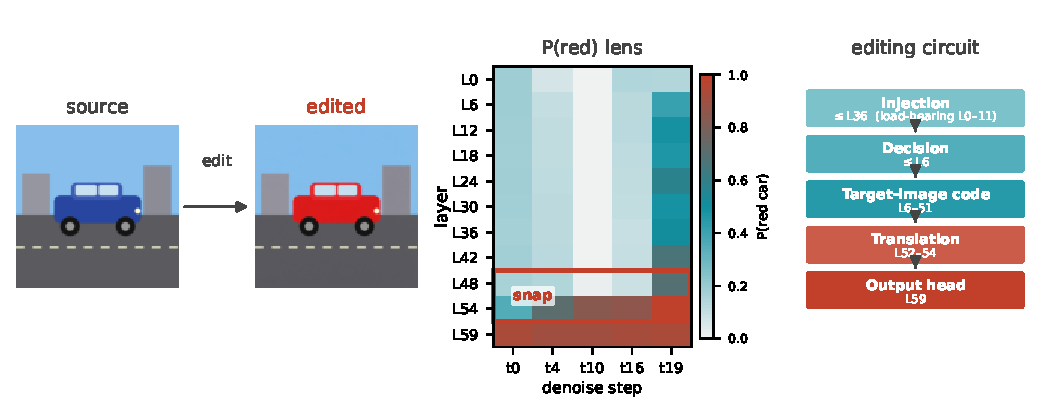
\includegraphics[width=0.98\textwidth]{figs/fig1_teaser.pdf}
  \caption{A layer--time lens for a DiT image editor. Decoding the
  frozen output head at intermediate layers of \emph{car\_red} gives a
  $P(\text{red car})$ grid across layer and denoising step (center); a
  sharp snap between layers 48 and 54 is where the head-readable
  signal first appears, but a linear probe shows the edit is already
  linearly decodable from layer 6. We read this as a five-stage
  \emph{editing circuit} (right): the instruction is injected early,
  the edit decision is linearly readable by layer 6, most of the stack
  then carries a target-image code, a narrow band (L52--54) translates
  it into the velocity code, and layer 59's frozen head reads it out --
  the edit is decided early and translated late, not developed
  gradually.}
  \label{fig:teaser}
\end{figure*}

% ===== AAAI-27 spine draft: Introduction (~0.9 col-page target) =====
\section{Introduction}\label{sec:intro}

Between reading ``turn the car red'' and painting it, what does a
diffusion image editor actually do? The mechanics of diffusion suggest
a gradual-development story, each of sixty blocks and twenty denoising
steps contributing its small share -- but this paper measures that
story and finds it wrong. In the model we study, the realized edit is
\emph{predictable early} from an internal target-image code, and only
\emph{translated late}, in the last few blocks, into the flow field that does
the painting.

Prior work provides partial readouts of generative internals. The logit and
tuned lenses project transformer residuals through a final or learned output
map~\citep{nostalgebraist2020logitlens,belrose2023tuned}. In diffusion,
Diffusion Lens interprets text-encoder states; DiffLens and ICM probe or steer
denoiser features; and DreamReader and sparse autoencoders provide broader
extraction and feature-analysis tools
~\citep{toker2024diffusionlens,shi2025difflens,zaleska2026icm,prakash2026dreamreader,surkov2025sae}.
Linear-representation work motivates a probe-readable basis, while multimodal
reasoners externalize visual thoughts as sketches or whiteboards
~\citep{park2024linear,hu2024sketchpad,menon2024whiteboard,wu2024vot,li2025mvot};
we instead test for an unrendered internal image, complementing the broader
thinking-with-images taxonomy~\citep{su2025thinkingsurvey}.
Recent work also detects early cross-seed convergence, predicts final quality
from early activations, or allocates adaptive image-editing budgets
~\citep{kwon2026lockin,guo2026probeselect,qu2026adecot}. None jointly decodes
an instruction-based DiT's image stream across both transformer depth and
denoising time while separating explicit-prompt readability from the realized
outcome under a fixed prompt.

A second line studies how to produce edits or intervene on hidden states.
Modern editors build on diffusion, latent/flow formulations, and guidance
~\citep{ho2020ddpm,song2021ddim,rombach2022ldm,lipman2023flowmatching,liu2023rectifiedflow,ho2022cfg}.
InstructPix2Pix and Prompt-to-Prompt learn or manipulate diffusion editing
controls~\citep{brooks2023instructpix2pix,hertz2023prompttoprompt}; ROME and
activation-patching practice transfer hidden states, while activation
engineering adds steering directions
~\citep{meng2022rome,heimersheim2024activation,turner2023actadd}. Concept
Lancet already uses representation transplant for diffusion editing
~\citep{luo2025colan}. Recent analyses further show that detectable diffusion
features can fail under steering and that multi-mediator patching can hide
interaction effects~\citep{cassano2026look,vaidyanathan2026curse}. We therefore
use transplant only as a sufficiency test and steering only as a bounded
writability test, not as a standalone editing method or a necessity proof.

We build a layer--time lens for a production DiT editor,
\model{} (60 blocks)~\citep{peebles2023dit,qwen2025image}, by decoding intermediate residual streams through
the model's own frozen output head, and -- crucially -- pair passive
readings with linear probes and controlled activation
interventions (ablation, transplant, steering) that test what those
activations can install or write.

Naively porting the logit-lens recipe reproduces the familiar mid-stack
``nothing happens yet'' appearance -- and that appearance is itself
misleading. With source and an underspecified recoloring instruction
fixed across 48 seeds, a generation-level probe predicts the color
ultimately chosen from layer 6, where the frozen head still reads noise.
The outcome is held in a basis the head cannot parse until a narrow band
near the top translates it into the velocity field that paints the result.

The main contributions of this work are as follows:
\begin{itemize}
\item \textbf{An instrument.} A layer--time instrument for a DiT image
editor, combining a training-free frozen-head lens with tuned and
differential variants,
paired with linear probes and three intervention primitives (ablate,
transplant, steer) with stated write semantics, under a
falsification-first protocol -- pre-registered predictions, per-image
visual verdicts, and bit-exact gates.
\item \textbf{A mechanism: the editor thinks with an internal image.}
The realized edit is predictable early under a fixed underspecified
instruction, carried as a target-image code, and translated into the
velocity code near layers 52--54. Across the two densely measured
timesteps, the crossover midpoint differs by under one layer while its
width varies from one to four layers; the boundary also replicates in a
same-lineage fine-tune and a 4-step distillation. Transplant establishes
sufficiency; in the tested recolor setting, steering and a rank ladder show
that readable attributes require a spatial carrier and a
variable-dependent write subspace.
\item \textbf{Validation and a lever.} Held-out early best-of-five selection
validates the readout on Qwen and an independent architecture, with about
68\% measured compute reduction. Separately, truncating classifier-free
guidance after step 2 saves 45\% of forward passes across tested edit
families; dropping CFG entirely produces failures consistent with a
non-redundant role in scope resolution rather than outcome selection.
\end{itemize}
This is exploratory, single-model-family work; every verdict was made
on the images themselves, and we are explicit about where the lens is
unreliable.


% ===== AAAI-27 spine draft: Related Work (~0.5 col) =====
\section{Related Work}\label{sec:related}

\paragraph{Logit and tuned lenses.} The logit
lens~\citep{nostalgebraist2020logitlens} projects intermediate residual
streams through a language model's frozen unembedding; the tuned
lens~\citep{belrose2023tuned} fits a small per-layer affine map instead.
We port both to a DiT editor -- staying on the frozen-head side for
honesty and crossing to the learned side only to render the internal
image -- with the linear representation
hypothesis~\citep{park2024linear} licensing the informative disagreement
between a frozen head and a probe.

\paragraph{Thinking with images, and diffusion interpretability.} A
growing line has multimodal models reason \emph{with} explicit
intermediate images~\citep{su2025thinkingsurvey,hu2024sketchpad}; we
supply the mechanistic complement, an image that exists \emph{latently}
inside a generative editor before any pixel is committed. The Diffusion
Lens~\citep{toker2024diffusionlens} decodes a text-to-image model's
\emph{text encoder}; we decode the editing DiT's own denoising stack
mid-generation, building on the flow-matching
formulation~\citep{lipman2023flowmatching} and classifier-free
guidance~\citep{ho2022cfg} that \model{}~\citep{qwen2025image,peebles2023dit}
uses.

\paragraph{Causal interpretability.} Causal tracing / ROME~\citep{meng2022rome}
patches activations between runs, the move behind our transplant;
\citet{heimersheim2024activation} catalogue the patching pitfalls that
motivate reporting ``readable'' and ``necessary'' separately, and
activation addition~\citep{turner2023actadd} is the steering primitive we
instantiate with a probe direction. Our semantic readout uses
CLIP~\citep{radford2021clip} for lack of a better zero-shot alternative.


% ===== AAAI-27 spine draft: Method (~1.3 col-page target) =====
\section{Proposed Method: A Layer--Time Lens and Intervention Probes}\label{sec:method}

Figure~\ref{fig:method} summarizes the full pipeline; here we specify each
component. We study \model{}, a 60-block DiT editor whose image stream
concatenates noisy target tokens with always-clean condition tokens. All
quantities below are read from the
\emph{post-block residual} of selected blocks via forward hooks,
captured in the model's native \texttt{bfloat16}: image-stream
activations reach absmax ${\sim}3{\times}10^{9}$ even at layer 0, so a cast
to \texttt{float16} silently overflows most elements to \texttt{inf}
(bf16 capture is a lossless copy, not a downcast).

\paragraph{Notation and layer--time readout.}
Let $h_{\ell,t}^{(i)}\!\in\!\mathbb{R}^{d}$ denote the post-block residual
after block $\ell\!\in\!\{0,\ldots,59\}$ at denoising step $t$, for
image-stream row $i$ (target patch, condition patch, or a hooked subset);
$h^{\mathrm{tar}}_{\ell,t}$ stacks the target-patch rows used for all
image-space readouts below (condition rows are captured only for explicitly
stated controls). A lens operator
$\mathcal{L}_{\ell,t}:\mathbb{R}^{n\times d}\!\to\!\mathbb{R}^{n\times64}$
maps these residuals to a target-grid velocity estimate $\tilde v_{\ell,t}$.
Logit- and Jacobian-style lenses in language models align internal states
with output units along depth and token position; a DiT patch has no
vocabulary, so we define a \emph{layer--time lens} as a map from
$(\ell,t)$ to an image and then a score on a fixed grid:
\begin{equation}
  I_{\ell,t}
  = \mathcal{V}\!\left(\Pi_t\!\left(
  \mathcal{L}_{\ell,t}(h^{\mathrm{tar}}_{\ell,t})\right)\right),
  \qquad
  \Pi_t(\tilde v)=x_t-\sigma_t\tilde v,
  \label{eq:lens-grid}
\end{equation}
where $\mathcal{V}$ is the frozen VAE decoder. We score a fixed edit-region
crop of $I_{\ell,t}$ with CLIP ViT-L/14~\citep{radford2021clip}. With
unit-normalized image and prompt-ensembled text embeddings $e_I,e_T$, and
CLIP's learned logit scale $\gamma$, the forced-choice probability over the
reported label bank $\{y_k\}$ is
\begin{equation}
  [\mathcal{M}_{\ell,t}]_k
  \;=\;
  \mathrm{softmax}_k\!\Bigl(
    \gamma\, e_T(y_k)^\top e_I(\mathrm{crop}(I_{\ell,t}))
  \Bigr).
  \label{eq:clip-readout}
\end{equation}
Figures~\ref{fig:teaser} and~\ref{fig:method} instantiate
\eqref{eq:lens-grid}--\eqref{eq:clip-readout}: the image-editor analogue of
lexical alignment grids in logit/Jacobian-lens visualizations, not a full
$\partial \mathbf{y}/\partial h$ (a donor-scalar Jacobian basis is tested in
the supplement and does not coincide with probe or write directions).

\paragraph{Lens operators.}
The \emph{time lens} uses the terminal head output at step $t$:
\begin{equation}
  \hat{x}_0(x_t,t) = x_t - \sigma_t\, v_\theta(x_t,t),
  \label{eq:time-lens}
\end{equation}
decoded through the VAE---what the model currently believes it will output.
The \emph{depth lens} asks the same question at intermediate depth by
re-invoking the model's frozen output head (non-affine
\texttt{AdaLayerNormContinuous} + linear \texttt{proj\_out}, bit-exact
whether invoked at layer 59 or earlier):
\begin{equation}
  v_{\ell,t} = \mathrm{Head}(h^{\mathrm{tar}}_{\ell,t}),
  \qquad
  \hat{x}_{0,\ell,t} = x_t - \sigma_t\, v_{\ell,t},
  \label{eq:depth-lens}
\end{equation}
then $I_{\ell,t}=\mathcal{V}(\hat{x}_{0,\ell,t})$.
Because \texttt{norm\_out} has no learned scale, rescaling $h^{\mathrm{tar}}_{\ell,t}$ to
the terminal norm is a no-op (raw vs.\ rescaled agree to
\texttt{max\_rel\_diff}$=0$); we use the raw head everywhere with a
standing self-consistency gate on every grid.
The \emph{tuned lens}~\citep{belrose2023tuned} fits a per-$(\ell,t)$ ridge map
from $d{=}3072$ hidden dimensions to the $64$-d conditional-pass velocity,
one dictionary per cell,
\begin{equation}
  \hat{v}_{\ell,t} = W_{\ell,t} h^{\mathrm{tar}}_{\ell,t} + b_{\ell,t},
  \quad
  W_{\ell,t} = V^\top H (H^\top H + \lambda I)^{-1},
  \label{eq:tuned-lens}
\end{equation}
after token-wise centering; $\lambda$ is chosen per cell on a held-out
$10\%$ \emph{token} split, distinct from zero-shot tests that hold out an
entire edit family and source image (hyperparameters in the supplement).
The \emph{differential lens} differences edit and control runs that share a
seed (step-0 latents are then bit-identical):
\begin{equation}
  D_{\ell,t}
  = \bigl|I^{\mathrm{edit}}_{\ell,t}
  - I^{\mathrm{ctrl}}_{\ell,t}\bigr|,
  \label{eq:diff-lens}
\end{equation}
isolating the internal edit plan when the unchanged prompt is a faithful
no-op; a control-fidelity gate on correlation with the source flags cases
where it is not.

\paragraph{Linear probes.}
Neither \eqref{eq:clip-readout} nor a lens image is itself a causal claim.
We additionally fit a lightweight probe
$p(y \mid h_{\ell,t}) = \mathrm{softmax}(W h_{\ell,t})$ on hidden states
(cross-seed evaluation), reading the same $(\ell,t)$ grid in label space
rather than pixel space---the basis mismatch against the frozen head in
\eqref{eq:depth-lens} is central to our mechanism results.

\paragraph{Intervention probes.}
Three forward-hook overwrites of the post-block residual test distinct
properties, applied identically to both CFG passes:
\begin{align}
  h &\leftarrow \mathbf{0}\ \text{or}\ \bar{h}
  && \text{(ablate: necessity stress test)}, \nonumber \\
  h^{(\mathrm{rec})} &\leftarrow h^{(\mathrm{don})}
  && \text{(transplant: sufficiency)}, \nonumber \\
  h &\leftarrow h + \alpha d
  && \text{(steer: linear writability)},
  \label{eq:interventions}
\end{align}
with $\alpha$ in units of per-row RMS and $d$ a probe direction; an empty
ablation spec reproduces the baseline bit-for-bit. Repeated ablation can
drive activations off-manifold, so we treat it only as a coarse stress test.

\paragraph{Protocol: predict, look, gate.} Three rules make the
\emph{reasoning} reproducible, not just the runs. \textbf{Predict, then
run}: every intervention was pre-registered; refutations are reported as
prominently as confirmations, and several headline results are
pre-registered predictions that failed informatively. \textbf{Look at
every image}: no verdict rests on CLIP alone -- every run carries a
per-image visual verdict recorded before the aggregates were read, and
where the two disagree the image wins. \textbf{Gate the instrument}: the
empty-ablation and raw-vs-rescaled checks are standing regressions re-run
per experiment. Porting the method to another editor needs only a
native-dtype residual hook, the frozen-head gate, and region-restricted
probes -- the recipe executed unchanged in the cross-model replication
below.


% ===== AAAI-27 spine draft: Decided early (~0.9 col) =====
\section{The Edit Is Decided Early}\label{sec:early}

\paragraph{In time.} If the edit surfaced progressively, the commit step
would be late and roughly uniform. Running the time lens over a battery of
10 cases across 5 edit categories, the step at which $P(\text{target})$
first reaches within $0.05$ of its final value is instead
\emph{edit-dependent} and mostly \emph{immediate}: color, background, and
style edits commit at step 0--2, and only a wholesale new-object
insertion (\emph{add\_boat}) commits as late as step 7. A finer
IoU-mask-based onset measurement over 20 cases shows the split is
categorical, not continuous: 18 of 20 -- spanning final-edit-area
fraction $0.003$ to $0.99$ -- onset at step 0 regardless of how large or
novel-looking the finished edit is, and no continuous proxy predicts the
delay (edge-novelty $\rho{=}0.24$, $p{=}0.30$; area $\rho{=}{-}0.44$,
running the \emph{wrong} way). Only the two edits that insert genuinely
novel structure with no existing pixels to build on -- \emph{add\_boat}
and \emph{add\_runner} -- start late.

\paragraph{In depth, the naive lens says ``late''.} The frozen depth lens
tells a different-looking story. Decoding \emph{car\_red}'s intermediate
layers through the model's own head, the edit becomes head-readable only
in a sharp snap between layers 48 and 54 of 60 -- exactly the familiar
mid-stack ``nothing happens yet'' appearance of an LLM logit lens.

\paragraph{But a probe reads it 40 layers earlier.} That appearance is
misleading. A 3-way cross-seed linear probe (which of three colors was
requested), fit on hidden states from one seed and evaluated on a
held-out seed, is already at $0.883$ accuracy at \textbf{layer 6}, step 4
-- five blocks into a 60-block network -- where the frozen head at the
identical cell reads only $P(\text{red car}){=}0.111$
(Fig.~\ref{fig:mechanism}). The earliest cell to cross $0.9$ is L36/step 0.
The decision is present far earlier than the head can read it; it is
simply held in a basis the head -- built for the network's final-layer
convention -- cannot parse until the last few blocks. Decided early, read
out late.

\paragraph{Where the instruction enters.} A complementary text-stream
ablation locates where the prompt is \emph{consumed}: zeroing the model's
text tokens in only the first 11 blocks garbles the whole scene, while
zeroing them after layer 36 barely dents the edit ($P(\text{red}){=}0.993$).
The instruction is fused into the image stream early and is functionally
complete by layer 36 -- the ``injection'' stage of the circuit in
Fig.~\ref{fig:teaser}, whose full text-band table is in the supplement.
Together with the probe, this gives the paper's five-stage picture:
injection ($\le$L36), decision ($\le$L6), a target-image code, translation
(L52--54), and the output head.


\begin{figure}[t]
  \centering
  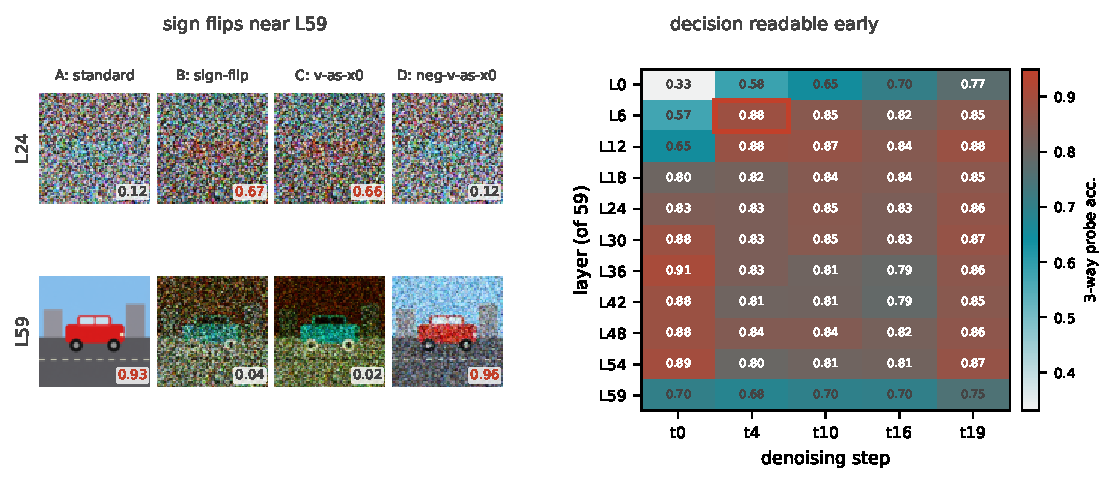
\includegraphics[width=\columnwidth]{figs/fig5_mechanism.pdf}
  \caption{Left: four ways of turning an intermediate layer's
  frozen-head output into an image for \emph{car\_red} at $t{=}4$ (A:
  standard $\hat{x}_0{=}x_t{-}\sigma_t v_\ell$; B: sign-flipped; C:
  $v_\ell$ decoded directly; D: $-v_\ell$ decoded directly) -- at L24
  the standard decode is wrong-colored while the sign-flipped/direct
  decodes already look red, and at L59 this reverses. Right: cross-seed
  3-way probe accuracy (chance $=0.33$) by layer/step; the headline
  cell L6/$t$4 ($0.883$) is far above the frozen-head reading at the
  same cell, and probe accuracy drops at L59 relative to L48--L54.}
  \label{fig:mechanism}
\end{figure}

% ===== AAAI-27 spine draft: Translated late / two codes (~1.6 col) =====
\section{The Edit Is Translated Late: Two Codes}\label{sec:translate}

If the decision is present by layer 6 but the frozen head cannot read it
until layer 52, the mid-stack must hold the edit in a \emph{different
code}. Three measurements show what that code is and where it is
converted.

\paragraph{Two decoding conventions cross over.} At an intermediate layer
the frozen head yields a per-token vector $v_\ell$ we normally treat as a
velocity, forming $\hat x_0 = x_t - \sigma_t v_\ell$ (variant A). Decoding
$v_\ell$ instead \emph{directly}, as if it were already a clean latent
(variant C), inverts the story: for \emph{car\_red} at step 4, at L24 the
standard decode A scores $P(\text{red}){=}0.12$ (still wrong-colored)
while the direct decode C already scores $0.66$; at L59 this reverses (A
$=0.93$, C $=0.02$). The mid-stack is not blank -- it encodes the target
content in an \emph{image-like} convention, and a narrow band near the top
reconciles it to the velocity convention the head consumes. (This is a
whole-vector reweighting, not a literal sign flip: essentially no
individual channel of $v_\ell$ has a negative slope against $v_{59}$, mean
$0.003$.)

\paragraph{The conversion is a sharp, timestep-invariant band.} A dense
every-layer sweep from L44 to L59 (Fig.~\ref{fig:boundary}) locates the
A/C crossover precisely: transition midpoint L53.6 at step 16 (width one
layer) and L52.7 at step 4, the two differing by under one layer -- the
boundary's \emph{location} is timestep-invariant. Crucially, the
cross-seed probe accuracy is close to \emph{flat} ($0.77$--$0.84$) across
every layer from L44 through L58 and drops only at the terminal layer L59
($0.68$--$0.70$). So the translation that changes what the head can read
(L52--54) and the loss of linear separability (L59) are two \emph{distinct}
events sharing a neighborhood: the target-image code survives the
translation intact and is degraded only by the final, velocity-specific
projection.

\paragraph{A tuned lens renders the internal image, layer by layer.} To
confirm the mid-stack code is a genuine \emph{image} rather than a probe
artifact, we fit a per-(layer, timestep) tuned lens
(\S\ref{sec:method}) on \emph{remove}/\emph{background}/\emph{addition}
edits and evaluate it \emph{zero-shot} on the held-out \emph{car\_red}
color family. Held-out $R^2$ rises with depth from $0.73$--$0.89$ at L6 to
$0.998$ at L59, where a standing identity gate confirms the target is
correct (decoding L59 through the frozen head reproduces the true velocity
bit-for-bit, max$|$diff$|{=}0$). Every depth down to L6 decodes a coherent
scene: a pre-registered prediction that readability itself would have a
boundary is refuted -- the L52--54 boundary is a property of the frozen
head's one fixed projection, not of the representation. At step 0 the
pixels are pure noise, so the decode comes entirely from the velocity
code, and we watch the edit enter the internal image directly
(Fig.~\ref{fig:tunedlens}): the source's blue car persists through L24,
turns orange-red by L36, the scene composes by L44, and the car is fully
red by L52. The same frozen dictionaries transfer with zero retraining to
six further held-out cases (style, more colors, removal, background,
addition); \emph{add\_runner} even reproduces the delayed onset on the
internal image's own time axis -- an empty path at step 0, a blurred
figure by step 2, a clear runner by step 4.

\paragraph{The anti-image, mechanized.} This also explains a striking
artifact: the mid-stack \emph{frozen}-head decode at later steps is a
color-\emph{inverted} ghost -- a cyan car under a red-brown sky, the exact
complement of the true scene. It is the image-like mid-stack code forced
through a head built to consume a velocity: $\hat x_0 = x_t - \sigma v$
flips the sign of an image-like quantity. The tuned lens at the same cell
is already coherent.


\begin{figure*}[t]
  \centering
  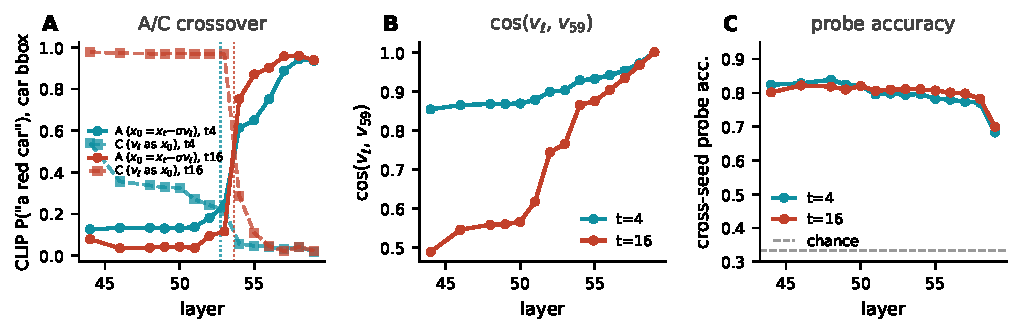
\includegraphics[width=0.98\textwidth]{figs/fig10_boundary.pdf}
  \caption{A dense, every-layer sweep of \emph{car\_red} over L44--L59
  sharpens the coarse L48/L54 snap to a precise boundary.
  \textbf{A}: the standard decode and the direct-$v$ decode cross
  between L52 and L54 at both steps shown. \textbf{B}: cosine
  similarity of the intermediate pseudo-velocity to the terminal
  $v_{59}$ rises sharply in the same band. \textbf{C}: cross-seed probe
  accuracy is flat from L44 through L58 and drops only at the terminal
  layer.}
  \label{fig:boundary}
\end{figure*}

\begin{figure*}[t]
  \centering
  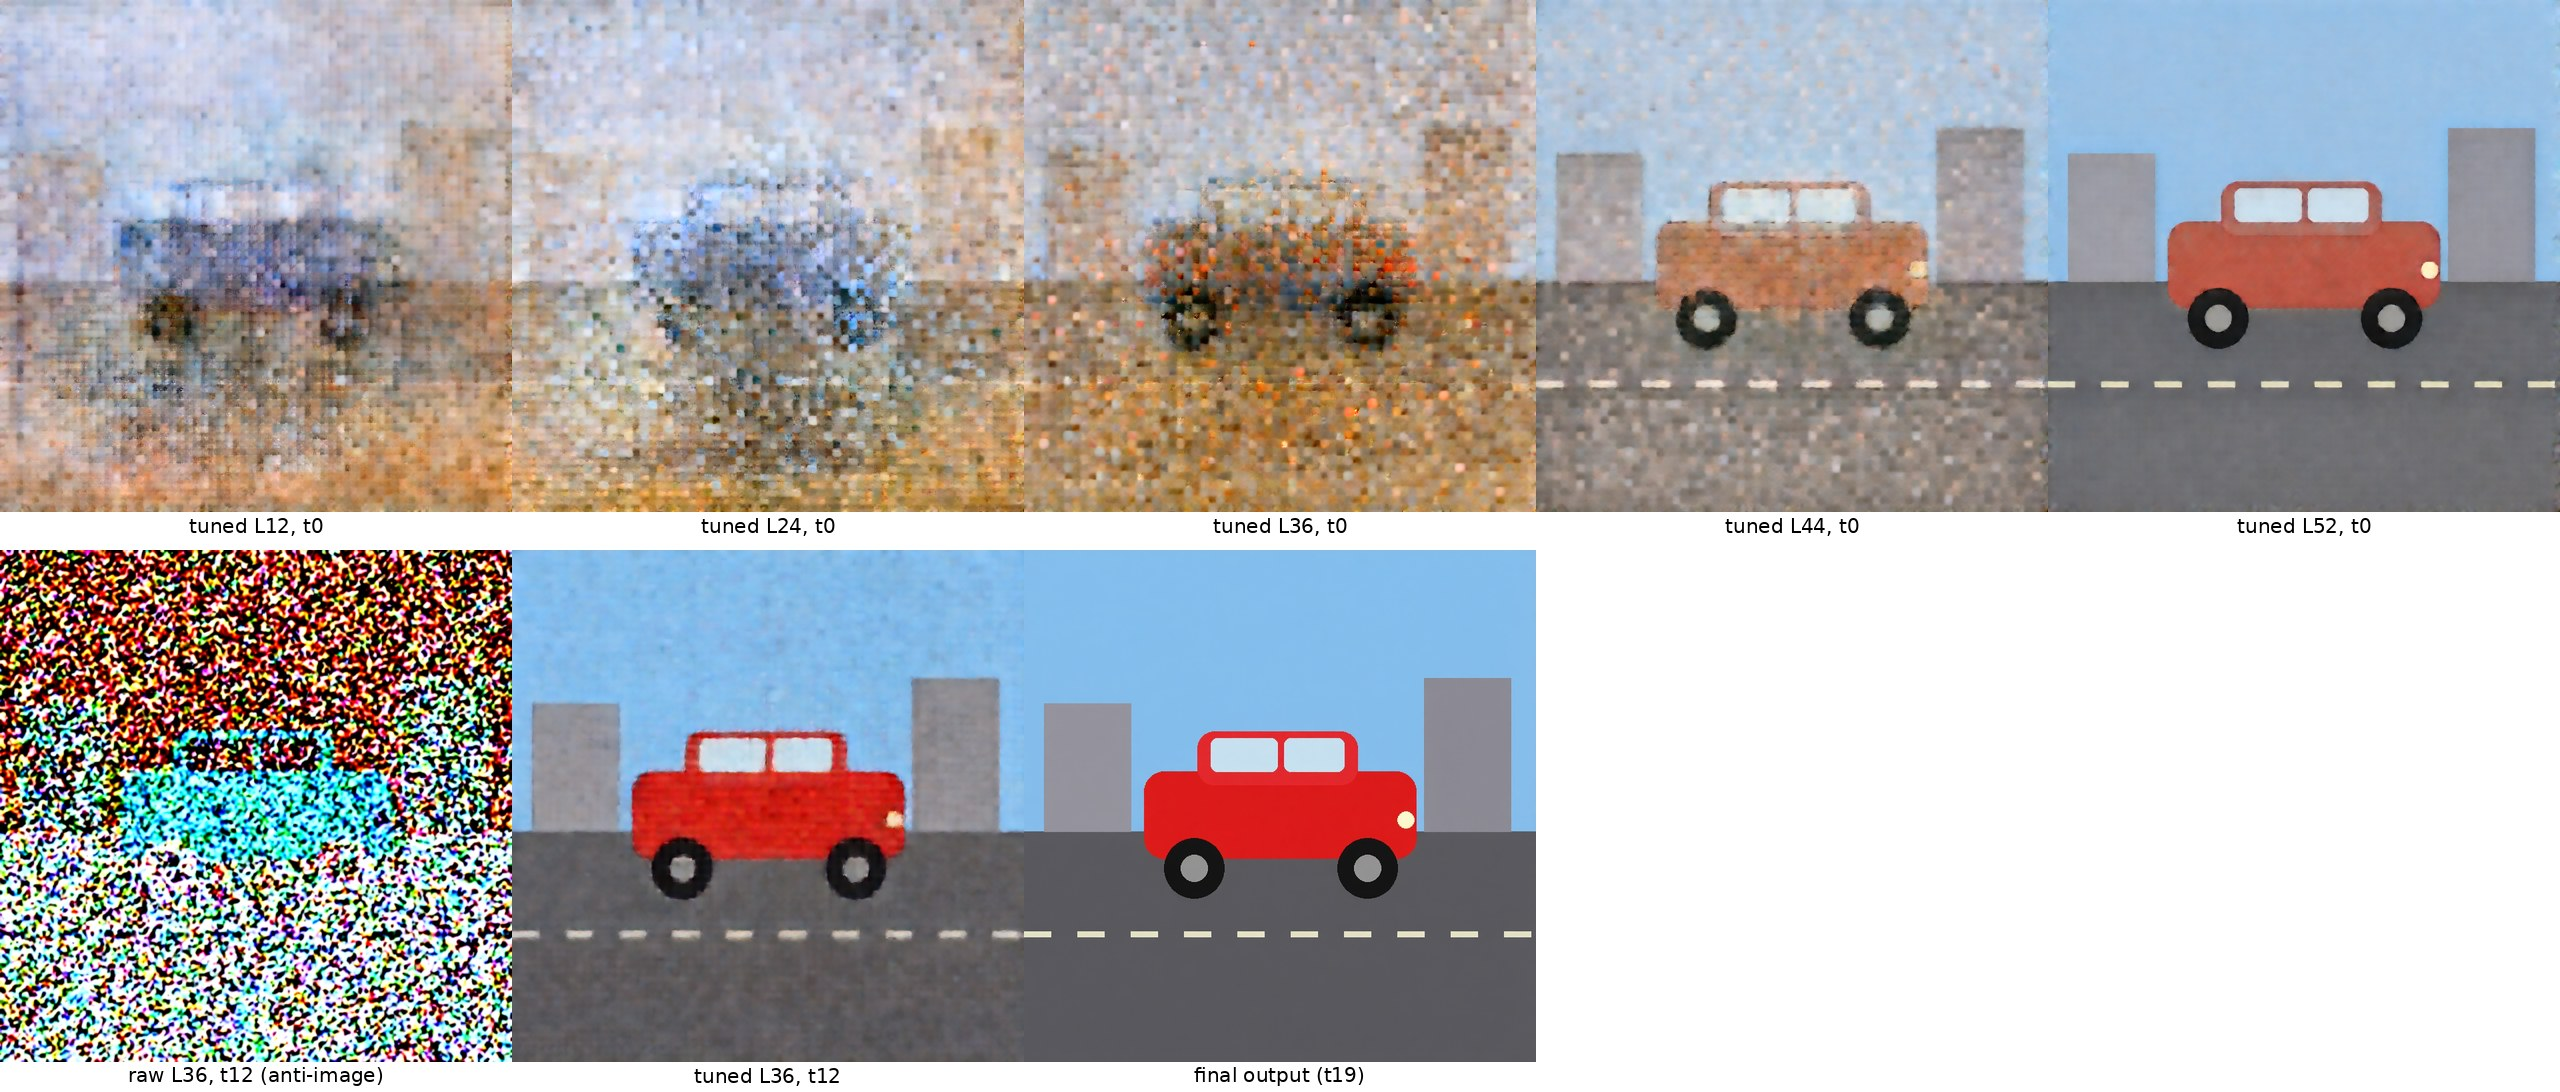
\includegraphics[width=0.98\textwidth]{figs/fig12_tuned_lens.jpg}
  \caption{A tuned lens renders the internal image the frozen head
  cannot read. Top: per-(layer, timestep) ridge translators, fit on
  \emph{remove}/\emph{background}/\emph{addition} edits and evaluated
  zero-shot on the held-out \emph{car\_red} color edit, decode a
  coherent scene at every depth at $t{=}0$, watching the edit enter the
  internal image layer by layer. Bottom: at $t{=}12$ the raw frozen
  head renders the identical L36 hidden state as a color-inverted
  ghost -- the complement of the true scene -- while the tuned lens at
  the same cell is already coherent.}
  \label{fig:tunedlens}
\end{figure*}

% ===== AAAI-27 spine draft: Three dissociations (~1.2 col) =====
\section{Readable, Necessary, Writable: Three Dissociations}\label{sec:dissoc}

Reading a lens shows only that a representation is \emph{consistent with}
an edit. Causal probes reveal that readability, causal necessity, and
linear writability are three different properties, and a layer band can
have any two without the third.

\paragraph{Readable $\neq$ necessary.} Ablating \emph{car\_red}'s early
layers (L0--11) is catastrophic ($P(\text{red}){=}0.049$) while ablating
the late band L48--59 is nearly harmless ($0.826$, versus an unablated
baseline near $0.93$) -- even though that late band is exactly where the
frozen head finally reads the edit. \emph{beach\_background} mirrors this
(L0--11 ablation only partial at $0.193$, L48--59 catastrophic at
$0.040$), and the split tracks commit time: the early-committing edit
needs early layers, the late-committing edit needs late ones
(Fig.~\ref{fig:causal}).

\paragraph{Sufficient $\neq$ necessary.} Transplanting a \emph{car\_red}
donor's car-region hidden states into a \emph{car\_green} recipient (which
alone scores $P(\text{red}){=}0.011$) flips the output to red from
\emph{any} of four donor bands -- including \textbf{L48--59} ($0.940$),
the very band ablation just showed is dispensable to the recipient. The
donor's late representation is \emph{sufficient} to install the edit even
where the recipient's own late computation is not \emph{necessary}. A
content control confirms specificity: splicing the same donor's
\emph{background}-region tokens (right band, wrong content) yields a
garbled ``blue car'' ($0.991$), not red.

\paragraph{Writable, but only onto a carrier.} A single stored
\emph{direction} -- the probe's $d_{\text{red}}$, no donor pass -- added to
the recipient's car rows gives a sharp sigmoidal dose-response ($0.024$ at
$\alpha{=}0.5$, $0.977$ at $\alpha{=}1$, saturating to $\alpha{=}8$); a
random direction of equal norm is inert ($0.017$), and the negated
direction overshoots to blue ($0.945$), reproducing the anti-image under
an active intervention. But writability is bounded: at effective doses the
steered region is not a recolored car but a flat red patch that
\emph{replaces} the car's geometry -- the direction installs \emph{which}
hue, not \emph{where to stop}. Supplying that missing ``where'' with the
edited object's own silhouette mask turns every previously-failing dose
into a clean in-place recolor. And conjuring an \emph{object} outruns any
single direction entirely: the probe direction for object identity is
inert, because the subspace a variable is read from and the subspace that
changes it are not the same -- a rank ladder over the donor$-$recipient
difference resolves identity coarse-to-fine (category at rank 1, a
coherent instance by rank 4, donor-faithful by rank 64, $2\%$ of the model
dimension). Readability, necessity, and writability thus dissociate three
distinct ways, and we map exactly where.


\begin{figure*}[t]
  \centering
  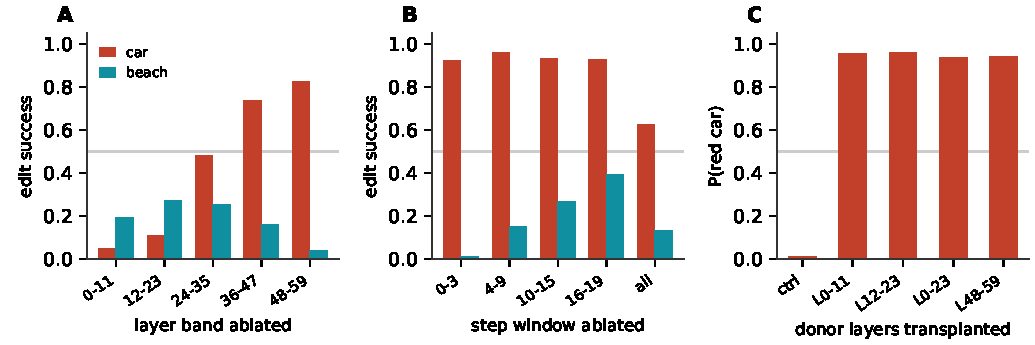
\includegraphics[width=0.98\textwidth]{figs/fig6_causality.pdf}
  \caption{Causal ablation and transplant, \emph{car\_red} vs.\
  \emph{beach\_background}. \textbf{A}: ablating a band of layers shows
  opposite profiles -- car needs its \emph{early} layers, beach needs
  its \emph{late} ones. \textbf{B}: ablating a window of steps shows
  car tolerates any single window, beach is destroyed by ablating the
  earliest one. \textbf{C}: transplanting a donor \emph{car\_red} run's
  hidden state into a \emph{car\_green} recipient, at any of four layer
  bands, is \emph{sufficient} to flip the output back to red --
  including the L48--59 band, which panel A shows is \emph{not
  necessary} for the car edit at all.}
  \label{fig:causal}
\end{figure*}

% ===== AAAI-27 spine draft: Differential lens + 15% preview (~0.85 col-page) =====
\section{A Differential Lens: Previewing the Edit at 15\% NFE}\label{sec:difflens}

The tuned lens renders the whole internal image; to isolate the
\emph{edit} from the reconstruction we difference it against a control.
We run the same source and seed twice -- once with the edit prompt, once
with the literal instruction ``keep the image unchanged'' -- and decode
both through the \emph{same} frozen dictionaries (no refit). Since the two
runs share a seed, their step-0 latents are bit-identical, so
$D_{\ell,t}=|\text{decode}(h_\ell^{\text{edit}})-\text{decode}(h_\ell^{\text{unchanged}})|$
isolates the internal edit plan, the reconstruction cancelling by
construction. This also answers \S\ref{sec:translate}'s open caveat that
the tuned lens's high $R^2$ might be easy background variance: token-level
$R^2$ \emph{inside} the edit region is $0.88$--$0.97$, matching the
full-image value -- the dictionaries carry the edit-specific signal
itself.

\paragraph{Commitment is early; separation is gradual.} A pre-registered
prediction that $D$ would already localize tightly at every step is
refuted, informatively. The edit \emph{content} is present at step 0 (the
tuned lens already shows red eyes, a black trunk), but the
\emph{differential} at step 0 is a diffuse whole-frame field -- the edit
prompt perturbs the entire velocity relative to the no-op, not just the
edited region -- and condenses onto the edit's footprint only gradually
(localization of $D$'s top mass at L52 climbs monotonically across steps,
e.g.\ $0.21{\to}0.47{\to}0.67{\to}0.83$ for a cat's-eyes recolor).
\emph{Committed} (is the content in the internal image) and
\emph{separated} (has the differential found where it lives) are two
different quantities, and the value of the no-op control is that it also
caught a case where the model \emph{cannot} do nothing -- one flat-art
scene rendered a transparent-PNG checkerboard for ``keep unchanged,''
which we discard, motivating a control-fidelity gate before any
differential number is trusted.

\paragraph{A preview lever.} Because the differential carries the edit's
footprint, we ask whether it does so early enough to be useful. At step 2
-- the third of 20, $\approx$15\% of the forward passes -- across a
10-case, five-family battery of natural photographs (all passing the
control-fidelity gate, $r\in[0.86,0.99]$), the median IoU between
$D_{\text{L52},t2}$'s top mass and the true edit region is $0.33$,
$6.6\times$ chance, and all 10 cases sharpen from step 0 to step 2
(Fig.~\ref{fig:previewlever}): an object slated for removal lights up as a
ghost, a keep-vs-replace background segmentation emerges unsupervised, and
a tiny recolor glows at its exact site. (Honestly, a fixed top-10\%
ground-truth mask under-scores genuinely tiny edits, padding their region
${\sim}10\times$ with collateral divergence -- a sixth documented
metric-vs-eye divergence in this work, and the first not caused by CLIP.)
Because the no-op control is \emph{independent of the edit prompt}, it can
be computed once per source image and cached; previewing where and how
large a \emph{candidate} edit will land then costs only the three forward
passes to reach step 2 plus one frozen-dictionary decode, not a full
20-step run -- a training-free way to triage many candidate prompts
against one image before committing to any.


\begin{figure}[t]
  \centering
  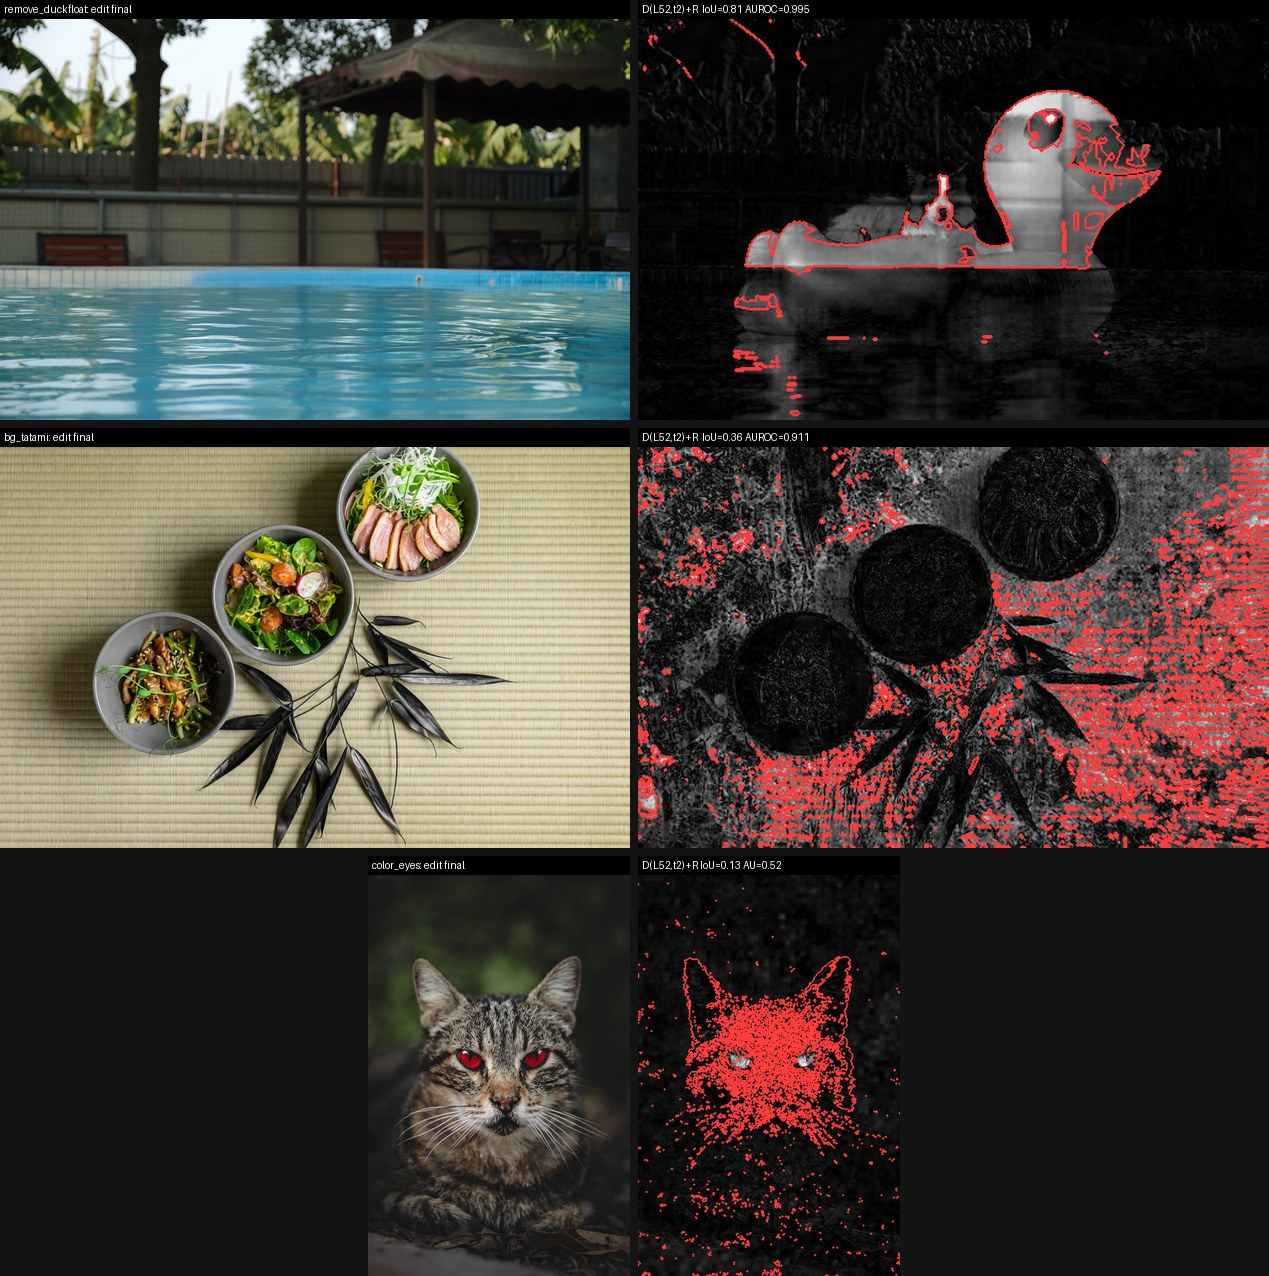
\includegraphics[width=\columnwidth]{figs/fig15_preview_lever.jpg}
  \caption{The differential lens as a $\approx$15\%-NFE ($t{=}2$) preview
  lever: three of a ten-case battery. Left: each case's final edited
  output. Right: the differential $D$ at layer 52, step 2, with the true
  edit region outlined in red -- an object slated for removal lights up as
  a ghost, a keep-vs-replace background segmentation emerges unsupervised,
  and a tiny recolor glows at its exact site, all at only 15\% of the
  denoising trajectory.}
  \label{fig:previewlever}
\end{figure}

% ===== AAAI-27 spine draft: Generalize + lever (~0.9 col) =====
\section{Does It Generalize? A Cross-Model Check}\label{sec:generalize}

Every finding so far concerns one checkpoint. We re-ran the depth-lens
crossover, the cross-seed probe, and layer-band ablation on two further
checkpoints sharing \model{}'s transformer classes: FireRed-Image-Edit-1.1,
an \emph{independent fine-tune}, and Rapid-AIO, a \emph{4-step distilled}
merge. \textbf{The translation boundary and the early decision replicate.}
FireRed's A/C crossover lands at L53--56, Rapid-AIO's at L52--54 -- both on
\model{}'s L52--54 band; FireRed's probe reads $0.852$ at L6 and dips to
$0.69$ at L59, the same flat-then-dip shape. \textbf{The decision direction
itself transfers across models}: a probe trained on one model and tested on
the \emph{other} reaches $0.84$/$0.92$ accuracy, and the two models'
L12 probe directions have cosine similarity $0.833$ -- the edit lives in
nearly the same direction of the shared 3072-d space, not merely the same
layer index. The full tuned-lens toolchain also ports to FireRed (deep-layer
$R^2$ $0.97$--$0.999$, anti-image reproduced). \textbf{One honest
divergence}, caught by the check doing its job: ablating L48--59 leaves
\model{}'s edit intact ($0.826$) but is catastrophic for FireRed ($0.035$)
-- late-stack redundancy is a property of \emph{training}, not the
architecture, so \S\ref{sec:dissoc}'s readable$\neq$necessary holds
architecture-generally only in its early half.

\section{A Lever: Truncating Classifier-Free Guidance}\label{sec:lever}

Because the decision is linearly present by layer 6 and translated by
layer 53, there is no architectural reason classifier-free guidance needs
both of its forward passes at all 20 steps. Running the unconditional pass
only for the first two steps and the conditional pass alone thereafter
leaves all four edit families visually intact at a \textbf{45\% reduction
in forward passes} (a 20-case battery confirms it, mean $1.77\times$
speedup). Dropping CFG entirely isolates its real job: recolor, removal,
and addition still land from the conditional pass alone, but background
swap composites the new scene \emph{around} un-erased source structure
($P(\text{beach}){=}0.45$ vs.\ ${\ge}0.996$) -- CFG's non-redundant
contribution is resolving \emph{scope}, not committing the edit. The same
decision structure survives $7.7\times$ step distillation (20/20 cases
land), so distillation compresses the sampling trajectory but not the
decision structure the lens exposes.


% ===== AAAI-27 spine draft: Limits + Conclusion (~0.8 col) =====
\section{Limitations and Honest Interpretation}\label{sec:limits}

This tool is exploratory. Every number comes primarily from one model,
one or two seeds, and a double-digit count of hand-chosen images; the
cross-model checks (\S\ref{sec:generalize}) cover two checkpoints of the
same lineage on a subset of measurements, and we make no claim about
``intent'' or about recovering the network's ``true'' reasoning. The
semantic readout inherits CLIP's failure modes in identifiable ways: pure
sampling noise can be mis-scored (a still-noisy decode labeled beach at
$0.795$), and, in mirror image, an obviously-red recolored car
\emph{under}-scores ($0.09$--$0.16$) while a \emph{failed} flat patch
scores higher ($0.70$--$0.84$) -- which is why every quantitative claim is
paired with a pre-registered visual verdict, and the image wins ties. Four
of our own initial misreadings are retained in the text as data: a
thumbnail ``revision'' phenomenon that quantification erased (leaving a
cleaner printing-vs-thinking split), a tempting continuous novelty law
that did not survive (only a categorical one did), a steering ``clean
flip'' that was a flat patch replacing the car's geometry, and the
over-strong conclusion we drew from it -- that a direction cannot carry
shape -- which a silhouette mask refuted. We claim only that, on \model{},
the readable/necessary/writable dissociations we report are real and
repeatable for the seeds and prompts used, because we checked them
against causal interventions rather than passive readouts alone.

\section{Conclusion}\label{sec:conclusion}

We built a layer--time and tuned lens for a 60-block DiT image editor and
paired every reading with a causal check. The edit is decided early
(linearly readable by layer 6), carried as a target-image code for most of
the depth, and translated into the velocity code only in a sharp,
timestep-invariant band at layer $\approx$53 -- a boundary that survives an
independent fine-tune and a 4-step distillation, while readability,
necessity, and writability dissociate three distinct ways. If one sentence
organizes the paper, it is this: \emph{the lens shows the translation, not
the decision -- reading the decision requires changing basis, and verifying
it requires intervention.} Behind it stands the picture we opened with and
have now earned clause by clause: an edit is not developed gradually -- it
is decided early, bound to a spatial carrier, and translated late into the
strokes that paint it. A generative editor natively thinks with an internal
image before it makes one; the lens turns that thought into something that
can be watched, steered, and budgeted for.


\bibliography{references}

\end{document}
